\textbf{Beispiel 3}\\ \\
a)\\ \\
RC-Ersatzschaltung:
\begin{figure}[h]
	\centering
	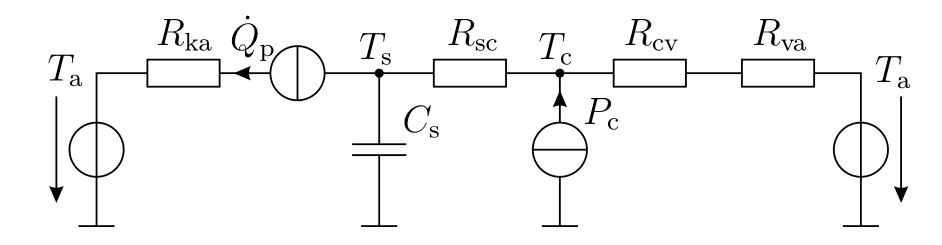
\includegraphics[width= 10cm]{tikz/16_03_2018_3a}
\end{figure}
\newline
Die Widerstände stellen die Wärmeübergänge, die Kapazität die Bereiche mit veränderlichen Temperaturen, die Stromquellen die Wärmeströme und die Spannungsquellen die konstanten Temperaturen dar.\\ \\
b)\\ \\
Die Chiptemperatur kann direkt aus der Ersatzschaltung bestimmt werden und lautet somit
\begin{align*}
	T_c(t) &= T_s(t) + \dot{Q}_{sc}R_{sc} = T_s(t) + \left(P_c + \frac{T_a - T_c(t)}{R_{cv} + R_{va}}\right)R_{sc}
\end{align*}
Durch Umformen erhält man
\[
	T_c(t) = \frac{T_s(t)(R_{cv} + R_{va}) + T_aR_{sc} + P_c(R_{cv} + R_{va}R_{sc})}{R_{sc} + R_{cv} + R_{va}}
\]
c)\\ \\
Die Temperaturänderung erfolgt nur durch die Wärmeströme über die Kapazität. Daher lautet die Differentialgleichung
\[
	\frac{\text{d}}{\text{d}t}T_s(t) = \frac{1}{C_s}(\dot{Q}_{sc} - \dot{Q}_p) =  \frac{1}{C_s}\left(P_c + \frac{T_a - T_c(t)}{R_{cv} + R_{va}} + \dot{Q}_p\right)
\]
\newpage
\noindent
d)\\ \\
Im stationären Fall verfällt die zeitliche Änderung, dadurch wird die Kapazität eine Unterbrechung und es ergibt sich für die gesuchten Temperaturen
\begin{align*}
	T_{c,\infty} &= T_a - (\dot{Q}_p - P_c)(R_{cv} + R_{va}) \\
	T_{s,\infty} &= T_{c,\infty} - R_{sc}\dot{Q}_p
\end{align*}
Diese Gleichungen wurden mithilfe der Ersatzschaltung aufgestellt. \\ \\